\begin{figure*}[ht!]
    \centering
    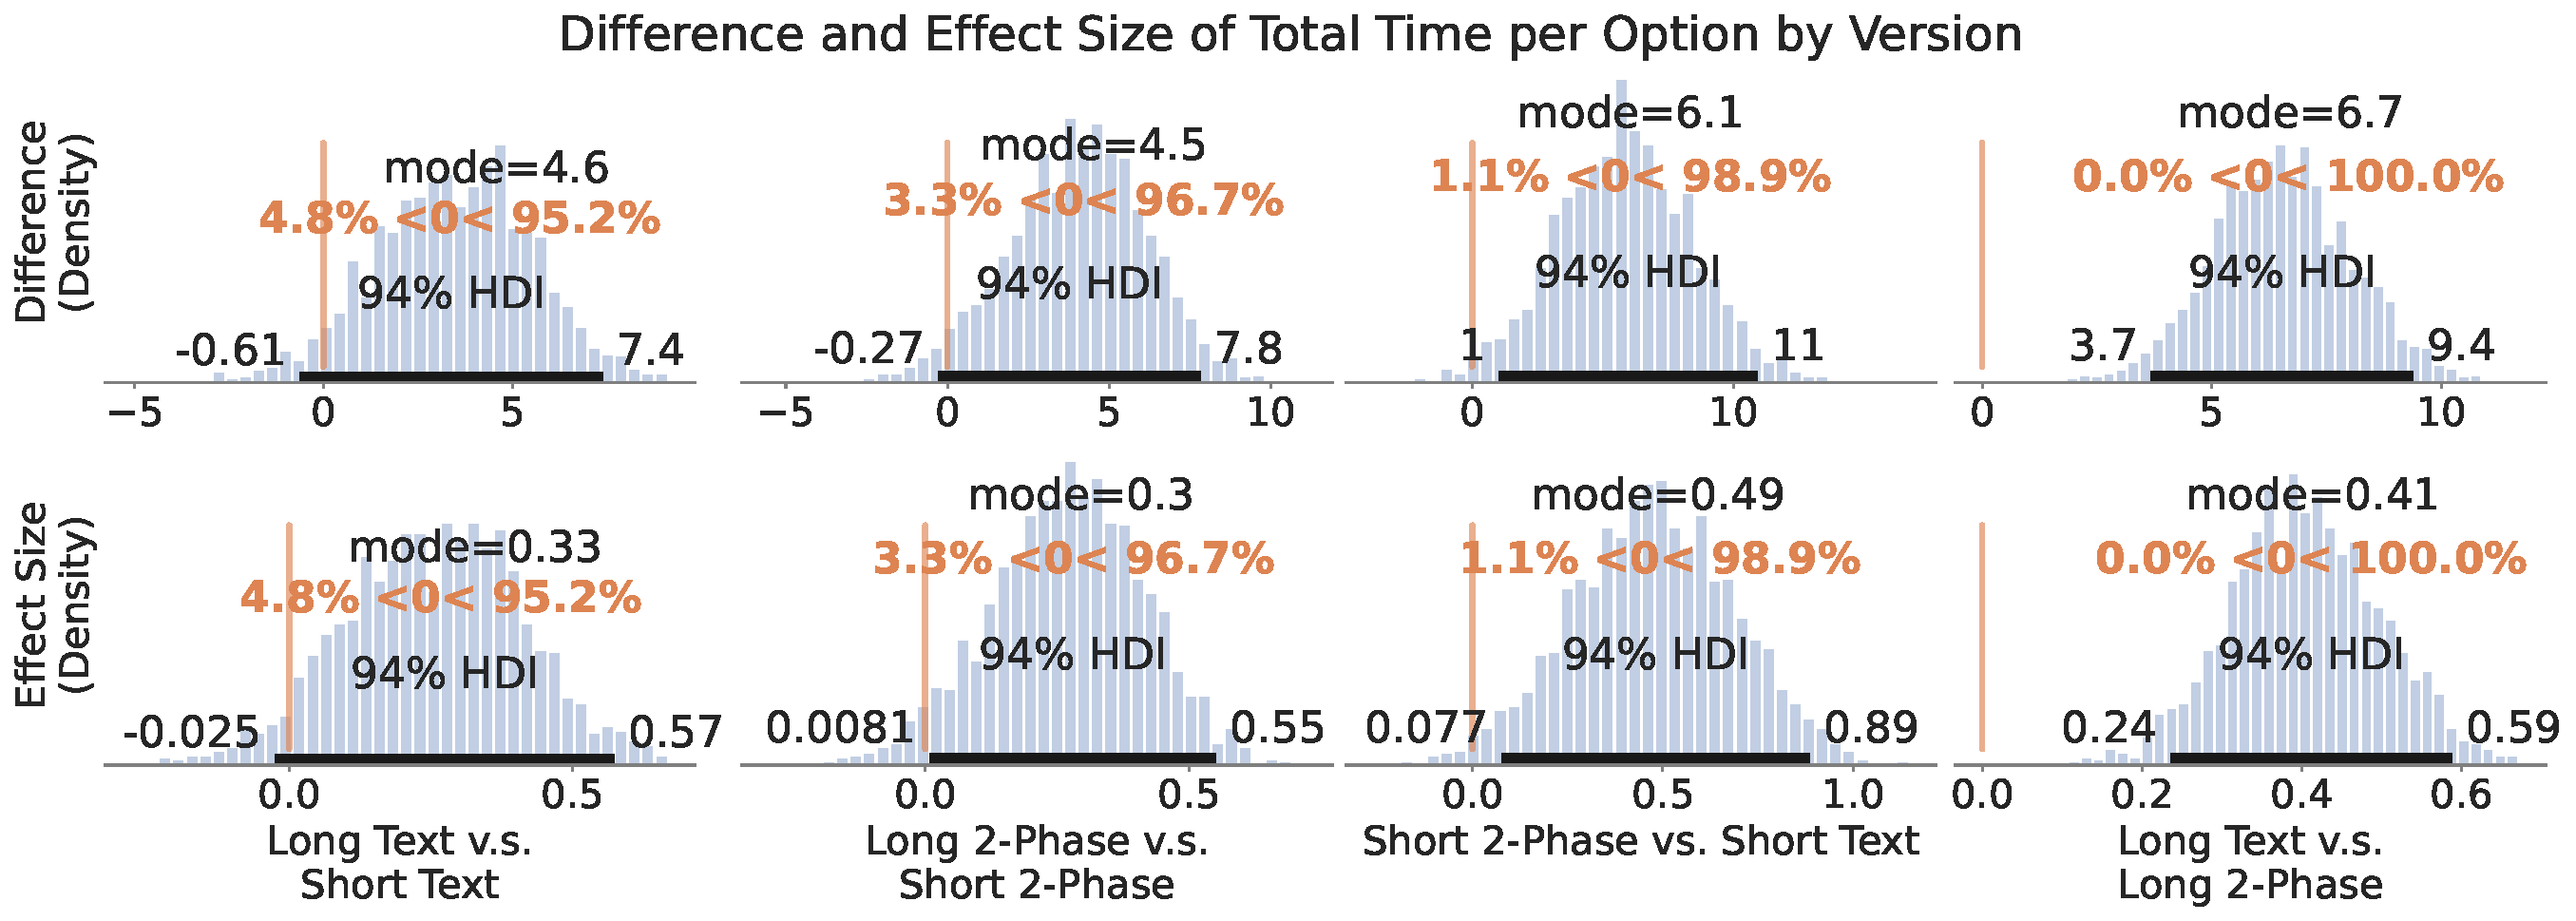
\includegraphics[width=0.75\textwidth]{content/image/time/time_diff_per_option_effect_size_by_version}
    % \captionsetup{width=0.9\textwidth, justification=justified}
    \caption{The figure shows the contrast distributions of the mean time to complete per option between pairwise experimental conditions, with the first row representing absolute differences and the second row depicting effect sizes.~\textbf{The main takeaway:} is that participants in the long two-phase condition spent more time per option compared to those in the long text and short two-phase conditions. Additionally, short two-phase participants took longer per option than short text participants.}
    \Description{ A grid of histograms titled "Difference and Effect Size of Total Time per Option by Version," showing posterior distributions of differences (top row) and effect sizes (bottom row) across four comparisons. Key values are annotated in orange, with vertical reference lines at zero indicating significance. The orange line between the Long and short two phase, between short 2 phase and text, and between long text and long two-phase are outside of the ROPE, indicating statistical differences in Bayesian terms.}
    \label{fig:time_per_option_bayesian}
\end{figure*}


\section{Clickstream data: Time participants spent}
\label{sec:timeAnalysis}
In addition to distance, participants in the short survey took an average of 2.7 minutes (short-text: $\mu=2.3$, $\sigma=1.27$; short two-phase: $\mu=3$, $\sigma=1.02$), while those in the long survey took 9.7 minutes (long-text: $\mu=7.5$, $\sigma=3.45$; long two-phase: $\mu=11.95$, $\sigma=2.73$). For a fairer comparison of interaction patterns, we analysis total ~\textbf{time-spend-per-option} using the QS system logs in this section. For participants in the two-phase interface conditions, this includes both organization and voting times for that option. The results are visualized in Figure~\ref{fig:total_time}.

Overall, participants spend slightly more time per option in the two-phase interface than in the text interface. To quantify these observations, we model the time data as predictive variables of separate Gamma distributions to characterize the continuous response times observed under distinct experimental conditions defined by survey length and interface type (Detailed in Appendix~\ref{sec:apdx:model_time}). Each of the four resulting subsets of data is modeled independently, with separate Gamma-distributed parameters governing the shape and rate of each group's time distributions. 

We calculated the posterior differences between the two-phase and text interfaces for all pairwise comparisons of the four groups. The results in Figure~\ref{fig:time_per_option_bayesian} indicate that participants using the two-phase interface consistently spend more time per option than those using the text interface, regardless of survey length. For both the short and long QSs, participants most likely spend 6.1 seconds (94\% HDI = [1.0, 11.0]) and 6.7 seconds (94\% HDI = [3.7, 9.4]) more per option, respectively, with medium effect sizes of $d=0.49$ (94\% HDI = [0.077, 0.89]) and $d=0.41$ (94\% HDI = [0.24, 0.59]). In both cases, the intervals lie outside the ROPE of 0 ± 1, indicating statistical significance. These findings suggest that the two-phase interface encourages longer deliberation, particularly for longer lists of options.

Some literature points to increased time can lead to cognitive fatigue~\cite{kundingerReliableGroundTruth2020, karim2024examining}, which can impair decision-making. Other decision science literature suggests that longer decision times can indicate deeper cognitive processing~\cite{payneAdaptiveDecisionMaker1993, daniel2017thinking}. Our qualitative analysis points to the latter.

Descriptively, participants in the long two-phase condition remained actively engaged during the voting phase, editing their votes an average of 39.3 times per participant ($\sigma=$39.3, range=$19-63$) compared to 39.1 times ($\sigma=$13.29, range=$15-58$) in the long text condition. This suggests that the two-phase interface does not reduce engagement despite the additional organization step.

Quantitatively, other than the difference in operational thinking and strategic consideration discussed in Section~\ref{sec:cog_diff}, we find that 37.5\% of participants (N=15) who attribute time to \textit{Decision Making} as a source of temporal demand frame such demand differently. We label a participant as \textit{affirmative} if they describe the pressure to make decisions as a source of temporal demand. For example, \smallquote{S022}{So it didn't take too much time, but obviously there were a lot of things to consider, so there was some temporal demand.} is an affirmative statement. Conversely, we label a participant as \textit{negative} if they express concern about the time and effort they have already invested. For example, \smallquote{S024}{maybe I should just hurry up and make a decision.} is a negative statement.


\begin{figure}[H]
    \centering
    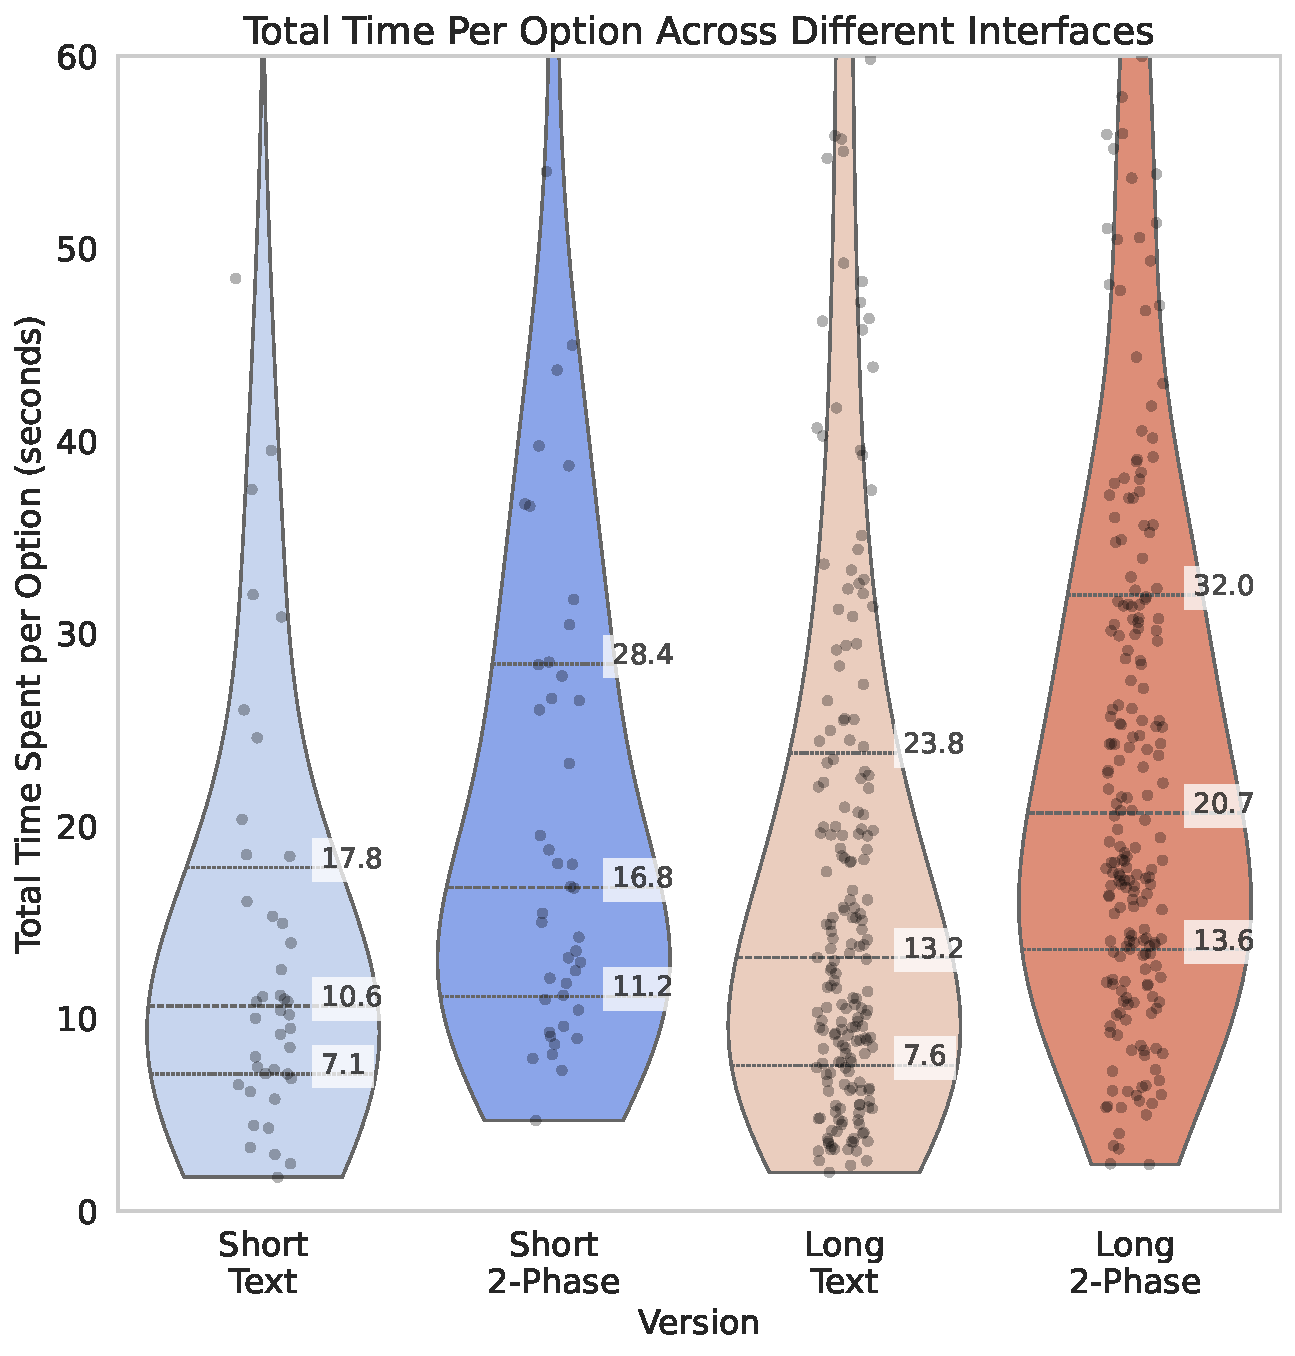
\includegraphics[width=0.45\textwidth, trim=0 0 0 0, clip]{content/image/time/Total Time Per Option Across Different Interfaces.pdf}
    % \captionsetup{width=0.45\textwidth, justification=justified}
    \caption{Total Time per Option. Each dot represents the time a participant took to complete an option, with the plot's shape showing the distribution within each group. The wider it is, the more dots there are. The three horizontal lines indicate the 25th, 50th, and 75th percentile annotated with value. The two-phase interface skewed slightly higher than the text interface~\textbf{Main takeaway: } Two-phase interface participants spend longer time per option compared to its counterparts.}
    \Description{Violin plot showing total time spent per option in seconds across four interface versions: Short Text, Short 2-Phase, Long Text, and Long 2-Phase. The y-axis ranges from 0 to 60 seconds. Each violin plot has scattered dots representing individual data points. The shape of the Short Text plot is widest between 10 and 20 seconds, tapering at the top and bottom. The Short 2-Phase plot is the narrowest, with most dots concentrated between 10 and 20 seconds. The Long Text plot is narrow and widest near the bottom, between 5 and 15 seconds. The Long 2-Phase plot is widest near the top, between 20 and 40 seconds.}
    \label{fig:total_time}
\end{figure}


50\% of participants (N=5) in the long two-phase group describe the pressure to make decisions affirmatively and none negatively. This suggests that their pressure stems from having too many remaining decisions to make, rather than from the time already invested. This is reflected in their higher average time spent per option and overall time spent ($\mu=716.86$ seconds, $\sigma=164.04$ seconds) completing the QS compared to the long text group ($\mu=449.64$ seconds, $\sigma=206.97$ seconds). We interpret results that participants are thoughtfully engaged in constructing their preferences and choose to invest additional time, rather than being driven by decision-related pressures or experiencing urgency.

% \begin{wrapfigure}[14]{r}{0.4\textwidth} % '14' adjusts vertical spacing if needed
%     \centering
%     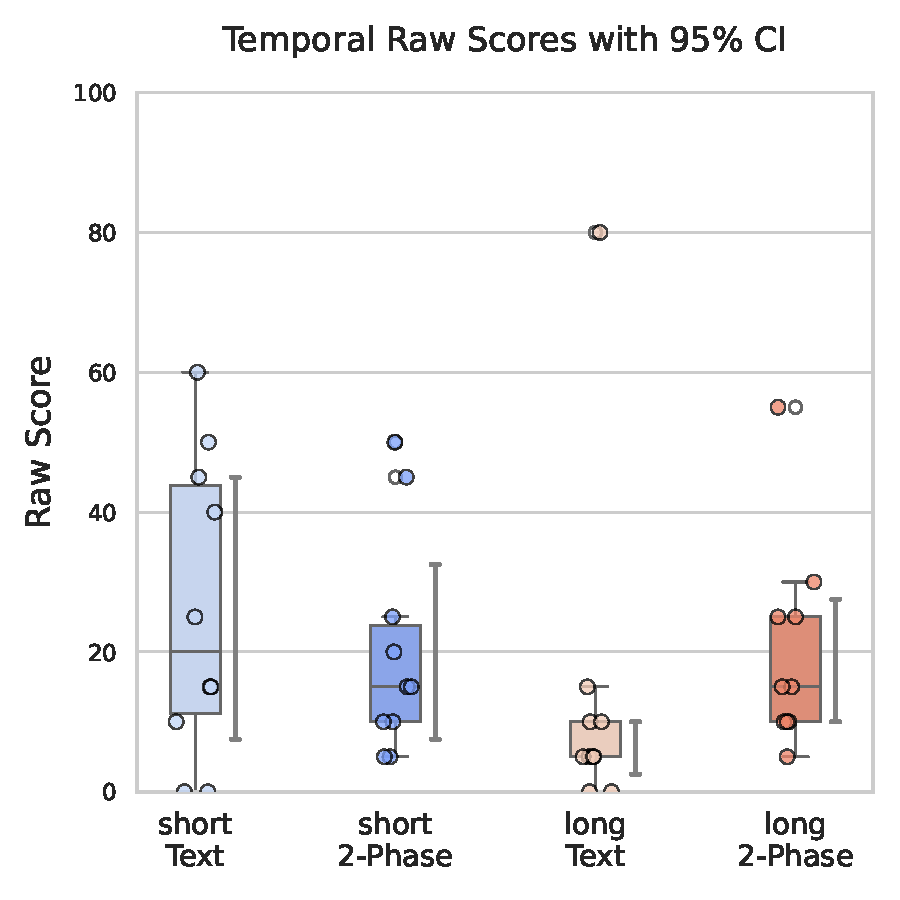
\includegraphics[width=\linewidth, trim=0 13 0 13, clip]{content/image/cog/Temporal_scores.pdf}
%     \captionsetup{width=0.95\linewidth, justification=justified} % Slightly narrower for better fitting
%     \caption{Temporal Demand Raw Score: Each dot represents a participant's subscale response.~\textbf{Main takeaway:} Long text interface participants seem to express less temporal demand compared to the other experiment conditions.}
%     \Description{A box plot titled "Temporal Raw Scores with 95\% CI," comparing raw temporal demand scores across four conditions: Short Text, Short 2-Phase, Long Text, and Long 2-Phase. Y-Axis represents 0 to 100 raw score, representing temporal demand. Short Text exhibited highest temporal demand with a wide spread of scores. Short 2-Phase showed moderate scores with reduced variability compared to Short Text. Long Text showed lowest temporal demand with minimal spread. Long 2-Phase showed moderate temporal demand, higher than Long Text but lower than Short Text. The plot shows boxplots with individual data points overlaid and whiskers indicating 95\% confidence intervals.}
%     \label{fig:temporal_cog_score}
% \end{wrapfigure}

Conversely, in the short text group, 50\% of participants (N=5) express concern about the time and effort they have already invested~(\smallquote{S024}{maybe I should just hurry up and make a decision.}) and none frame it affirmatively. Descriptively, participants in the short text group spend comparatively less time than those in the long QS (short text: $\mu=139.83$ seconds, $\sigma=76.43$ seconds; short two-phase: $\mu=178.78$ seconds, $\sigma=61.07$ seconds). This suggests that participants in the short text group expect themselves to complete the task sooner than they actually do. 

\begin{figure}[h]
    \centering
    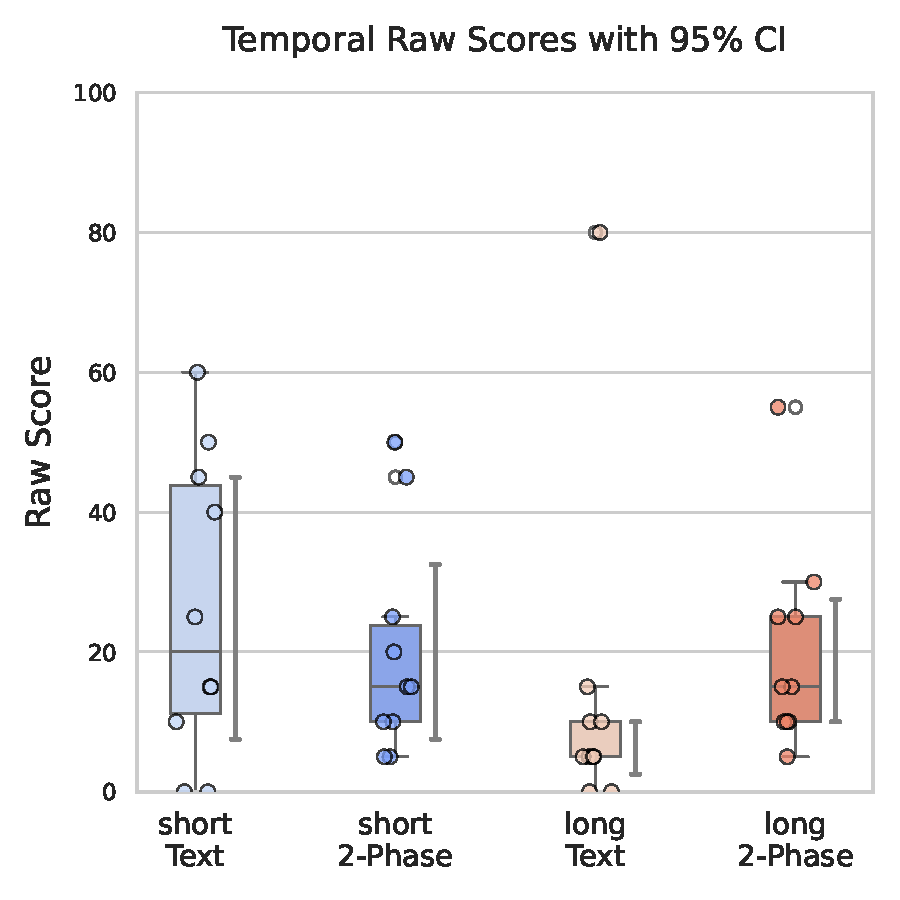
\includegraphics[width=0.4\textwidth, trim=0 13 0 13, clip]{content/image/cog/Temporal_scores.pdf}
%     \captionsetup{width=0.4\textwidth, justification=justified}
    \caption{Temporal Demand Raw Score: Each dot represents a participant's subscale response.~\textbf{Main takeaway:} Long text interface participants seem to express less temporal demand compared to the other experiment conditions.}
    \Description{A box plot titled "Temporal Raw Scores with 95\% CI," comparing raw temporal demand scores across four conditions: Short Text, Short 2-Phase, Long Text, and Long 2-Phase. Y-Axis represents 0 to 100 raw score, representing temporal demand. Short Text exhibited highest temporal demand with a wide spread of scores. Short 2-Phase showed moderate scores with reduced variability compared to Short Text. Long Text showed lowest temporal demand with minimal spread. Long 2-Phase showed moderate temporal demand, higher than Long Text but lower than Short Text. The plot shows boxplots with individual data points overlaid and whiskers indicating 95\% confidence intervals.}
    \label{fig:temporal_cog_score}
\end{figure}

Surprisingly, participants in the long text interface exhibit lower temporal demand compared to both the short text and long two-phase interfaces (Figure~\ref{fig:temporal_cog_score}). Bayesian analysis (Appendix~\ref{sec:temporal_subscale_bayesian}) supports this finding, with posterior probabilities of 86.1\% and 86.7\%, respectively. This result is notable considering participants spent more time per option compared to those in the short text interface and traversed the longest distance among all three groups (Section~\ref{dist}). In addition, only 30\% of participants (N=3) mention the time spent making a decision as a source of temporal demand. One possible explanation is that some participants are satisficing, as we pointed out in Section~\ref{sec:satisficing}.  

In summary, we interpret the result that participants in the two-phase interface spend more time per option as a sign of deeper cognitive processing. This is further supported by examining participants' nuanced voting behaviors under budget constraint conditions for the long QS, which we omit for brevity. Notably, two-phase interface participants make more small vote adjustments (i.e., adding or removing at most 2 votes on an option) when they have fewer remaining credits, further supporting our claim that they experience deeper engagement with preference construction, which we elaborate on further in Appendix~\ref{apdx:additional_results_behavior}.
